%%%%%%%%%%%%%%%%%%%%%%%%%%%%%%%%%%%%%%%%%
% Journal Article
% LaTeX Template
% Version 2.0 (February 7, 2023)
%
% This template originates from:
% https://www.LaTeXTemplates.com
%
% Author:
% Vel (vel@latextemplates.com)
%
% License:
% CC BY-NC-SA 4.0 (https://creativecommons.org/licenses/by-nc-sa/4.0/)
%
% NOTE: The bibliography needs to be compiled using the biber engine.
%
%%%%%%%%%%%%%%%%%%%%%%%%%%%%%%%%%%%%%%%%%

%----------------------------------------------------------------------------------------
%	PACKAGES AND OTHER DOCUMENT CONFIGURATIONS
%----------------------------------------------------------------------------------------

\documentclass[
	a4paper, % Paper size, use either a4paper or letterpaper
	10pt, % Default font size, can also use 11pt or 12pt, although this is not recommended
	unnumberedsections, % Comment to enable section numbering
	twoside, % Two side traditional mode where headers and footers change between odd and even pages, comment this option to make them fixed
]{LTJournalArticle}

\addbibresource{sample.bib} % BibLaTeX bibliography file

% \runninghead{Shortened Running Article Title} % A shortened article title to appear in the running head, leave this command empty for no running head

% \footertext{\textit{Journal of Biological Sampling} (2024) 12:533-684} % Text to appear in the footer, leave this command empty for no footer text

\setcounter{page}{1} % The page number of the first page, set this to a higher number if the article is to be part of an issue or larger work

%----------------------------------------------------------------------------------------
%	TITLE SECTION
%----------------------------------------------------------------------------------------

\title{Film Emulation Using Dynamic Range and Tone Mapping [TENTATIVE]} % Article title, use manual lines breaks (\\) to beautify the layout

% Authors are listed in a comma-separated list with superscript numbers indicating affiliations
% \thanks{} is used for any text that should be placed in a footnote on the first page, such as the corresponding author's email, journal acceptance dates, a copyright/license notice, keywords, etc
\author{%
	Christian Johnson\textsuperscript{1}, Alex Martin\textsuperscript{2} 
}

% Affiliations are output in the \date{} command
\date{\footnotesize\textsuperscript{\textbf{1}}Harvey Mudd College, \texttt{chrjohnson@hmc.edu} \\ \textsuperscript{\textbf{2}}Harvey Mudd College, \texttt{almartin@hmc.edu}}

% % Full-width abstract
% \renewcommand{\maketitlehookd}{%
% 	\begin{abstract}
% 		\noindent Lorem ipsum dolor sit amet, consectetur adipiscing elit. Praesent porttitor arcu luctus, imperdiet urna iaculis, mattis eros. Pellentesque iaculis odio vel nisl ullamcorper, nec faucibus ipsum molestie. Sed dictum nisl non aliquet porttitor. Etiam vulputate arcu dignissim, finibus sem et, viverra nisl. Aenean luctus congue massa, ut laoreet metus ornare in. Nunc fermentum nisi imperdiet lectus tincidunt vestibulum at ac elit. Nulla mattis nisl eu malesuada suscipit. Aliquam arcu turpis, ultrices sed luctus ac, vehicula id metus. Morbi eu feugiat velit, et tempus augue. Proin ac mattis tortor. Donec tincidunt, ante rhoncus luctus semper, arcu lorem lobortis justo, nec convallis ante quam quis lectus. Aenean tincidunt sodales massa, et hendrerit tellus mattis ac. Sed non pretium nibh. Donec cursus maximus luctus. Vivamus lobortis eros et massa porta porttitor.
% 	\end{abstract}
% }

%----------------------------------------------------------------------------------------

\begin{document}

\maketitle % Output the title section

%----------------------------------------------------------------------------------------
%	ARTICLE CONTENTS
%----------------------------------------------------------------------------------------

\section{Motivation}

When taking an image with a camera, the range of light and dark values it can represent at once is its dynamic range, with values outside of this range being completely dark or completely light, thus possessing no visual information. Dynamic range is a common complication for computational photography and image processing, as scenes with a wide range of light and dark (such as a sunset) become difficult to photograph properly with a consumer camera, as its limited dynamic range will make it challenging to to get bright areas and dark areas properly exposed to make a compelling image.

One popular approach to dealing with this problem is high dynamic range (HDR) photography, in which a series of computational techniques are used to generate an image with a dynamic range much higher than that of a single input photo. There are many approaches to creating an HDR image, with Deep Learning becoming an increasingly popular area, but the most widely used approach is image composition. In this method multiple images of the same scene are taken at different exposures, and then digitally combined to create a single image where areas of under/over exposure are filled in by the full set of images.

The result, however, is not yet a compelling photograph. Most displays and printing mediums are not designed for HDR images, and thus the wide range of exposure information will make the image seem low-contrast and dull. To correct this a technique called tone mapping is used, in which an HDR image is normalized and adjusted to match the contrast needs of displays while preserving the details and balance developed in the composite. In this process it is possible to replicate the exposure response of different film stocks, allowing us to use HDR imaging to emulate the look of color film photographs using digital cameras.

From this, our project will consist of two primary components: registration of multiple exposure images to form an HDR image, and tone mapping to emulate film photographs from HDR images.

%------------------------------------------------

\section{Technical Background}

There are a variety of algorithms for HDR compositing, but a popular choice and one available in OpenCV is the Debevec algorithm, that leverages a camera response curve to combine exposures – the response curve being the camera’s sensitivity to different amounts of light depending on exposure settings. By taking this into account the method works to reconstruct the original light levels of the scene unaffected by the camera’s response curve.

For the tone mapping we effectively conduct the opposite of the HDR composite production, in which we get the response curve to a chosen color film stock, and apply it to the HDR composite to get an image representative of a film stock’s response to the original scene. This work can be supplemented by the addition of glare and diffusion (with one such example coming from Debevec’s paper) to more accurately recreate the look that a film stock would produce when exposed to the scene.

As a final note we plan to use the RAW files from a Sony digital camera, to give us the most exposure and image data possible.

For the tone mapping we effectively conduct the opposite of the HDR composite production, in which we get the response curve to a chosen color film stock, and apply it to the HDR composite to get an image representative of a film stock’s response to the original scene. This work can be supplemented by the addition of glare and diffusion (with one such example coming from Debevec’s paper) to more accurately recreate the look that a film stock would produce when exposed to the scene.

As a final note we plan to use the RAW files from a Sony digital camera, to give us the most exposure and image data possible.


\subsection{Methodology}

Our proposed methodology for HDR film emulation is as follows,
\begin{itemize}
	\item Collect a series of photographs of a scene with a wide range of light values (such as a sunset) at different exposure settings.
	\item Register the photos to fix any discrepancies in camera movement across the photos.
	\item Calculate an image response curve for the photos and compare it to the known response curve of the camera.
	\item Using the response curve and the registered images, use the Debevec algorithm to calculate an HDR composite.
	\item Recreate the image response curves of a film stock of choice.
	\item Use tone mapping with the film response curve (also known as a histogram transformation) to get a fill emulated image.
\end{itemize}
The folowing components are stretch goals,
\begin{itemize}
	\item Apply the methods of Ward Et al. to simulate the glare and contrast sensitivity of the film stock.
	\item Use edge detection on a radiance map of the HDR image to simulate halation – a tinted glow in overexposed film images.
	\item Use the color spectrum response of the film stock to modify the color response of the image to better match that of a film image. 
\end{itemize}
The majority of this work can be completed using OpenCV, with the assistance of some custom generated functions to allow for the tone mapping. The result of these steps should be a compelling and accurate emulation of a film image.

%------------------------------------------------

% \section{Results}

% \begin{table} % Single column table
% 	\caption{Example single column table.}
% 	\centering
% 	\begin{tabular}{l l r}
% 		\toprule
% 		\multicolumn{2}{c}{Location} \\
% 		\cmidrule(r){1-2}
% 		East Distance & West Distance & Count \\
% 		\midrule
% 		100km & 200km & 422 \\
% 		350km & 1000km & 1833 \\
% 		600km & 1200km & 890 \\
% 		\bottomrule
% 	\end{tabular}
% 	\label{tab:distcounts}
% \end{table}

% Referencing a table using its label: Table \ref{tab:distcounts}.

% \begin{table*} % Full width table (notice the starred environment)
% 	\caption{Example two column table with fixed-width columns.}
% 	\centering % Horizontally center the table
% 	\begin{tabular}{L{0.2\linewidth} L{0.2\linewidth} R{0.15\linewidth}} % Manually specify column alignments with L{}, R{} or C{} and widths as a fixed amount, usually as a proportion of \linewidth
% 		\toprule
% 		\multicolumn{2}{c}{Location} \\
% 		\cmidrule(r){1-2}
% 		East Distance & West Distance & Count \\
% 		\midrule
% 		100km & 200km & 422 \\
% 		350km & 1000km & 1833 \\
% 		600km & 1200km & 890 \\
% 		\bottomrule
% 	\end{tabular}
% \end{table*}

% Aenean feugiat pellentesque venenatis. Sed faucibus tristique tortor vel ultrices. Donec consequat tellus sapien. Nam bibendum urna mauris, eget sagittis justo gravida vel. Mauris nisi lacus, malesuada sit amet neque ut, venenatis tempor orci. Curabitur feugiat sagittis molestie. Duis euismod arcu vitae quam scelerisque facilisis. Praesent volutpat eleifend tortor, in malesuada dui egestas id. Donec finibus ac risus sed pellentesque. Donec malesuada non magna nec feugiat. Mauris eget nibh nec orci congue porttitor vitae eu erat. Sed commodo ipsum ipsum, in elementum neque gravida euismod. Cras mi lacus, pulvinar ut sapien ut, rutrum sagittis dui. Donec non est a metus varius finibus. Pellentesque rutrum pellentesque ligula, vitae accumsan nulla hendrerit ut.

% \begin{figure} % Single column figure
% 	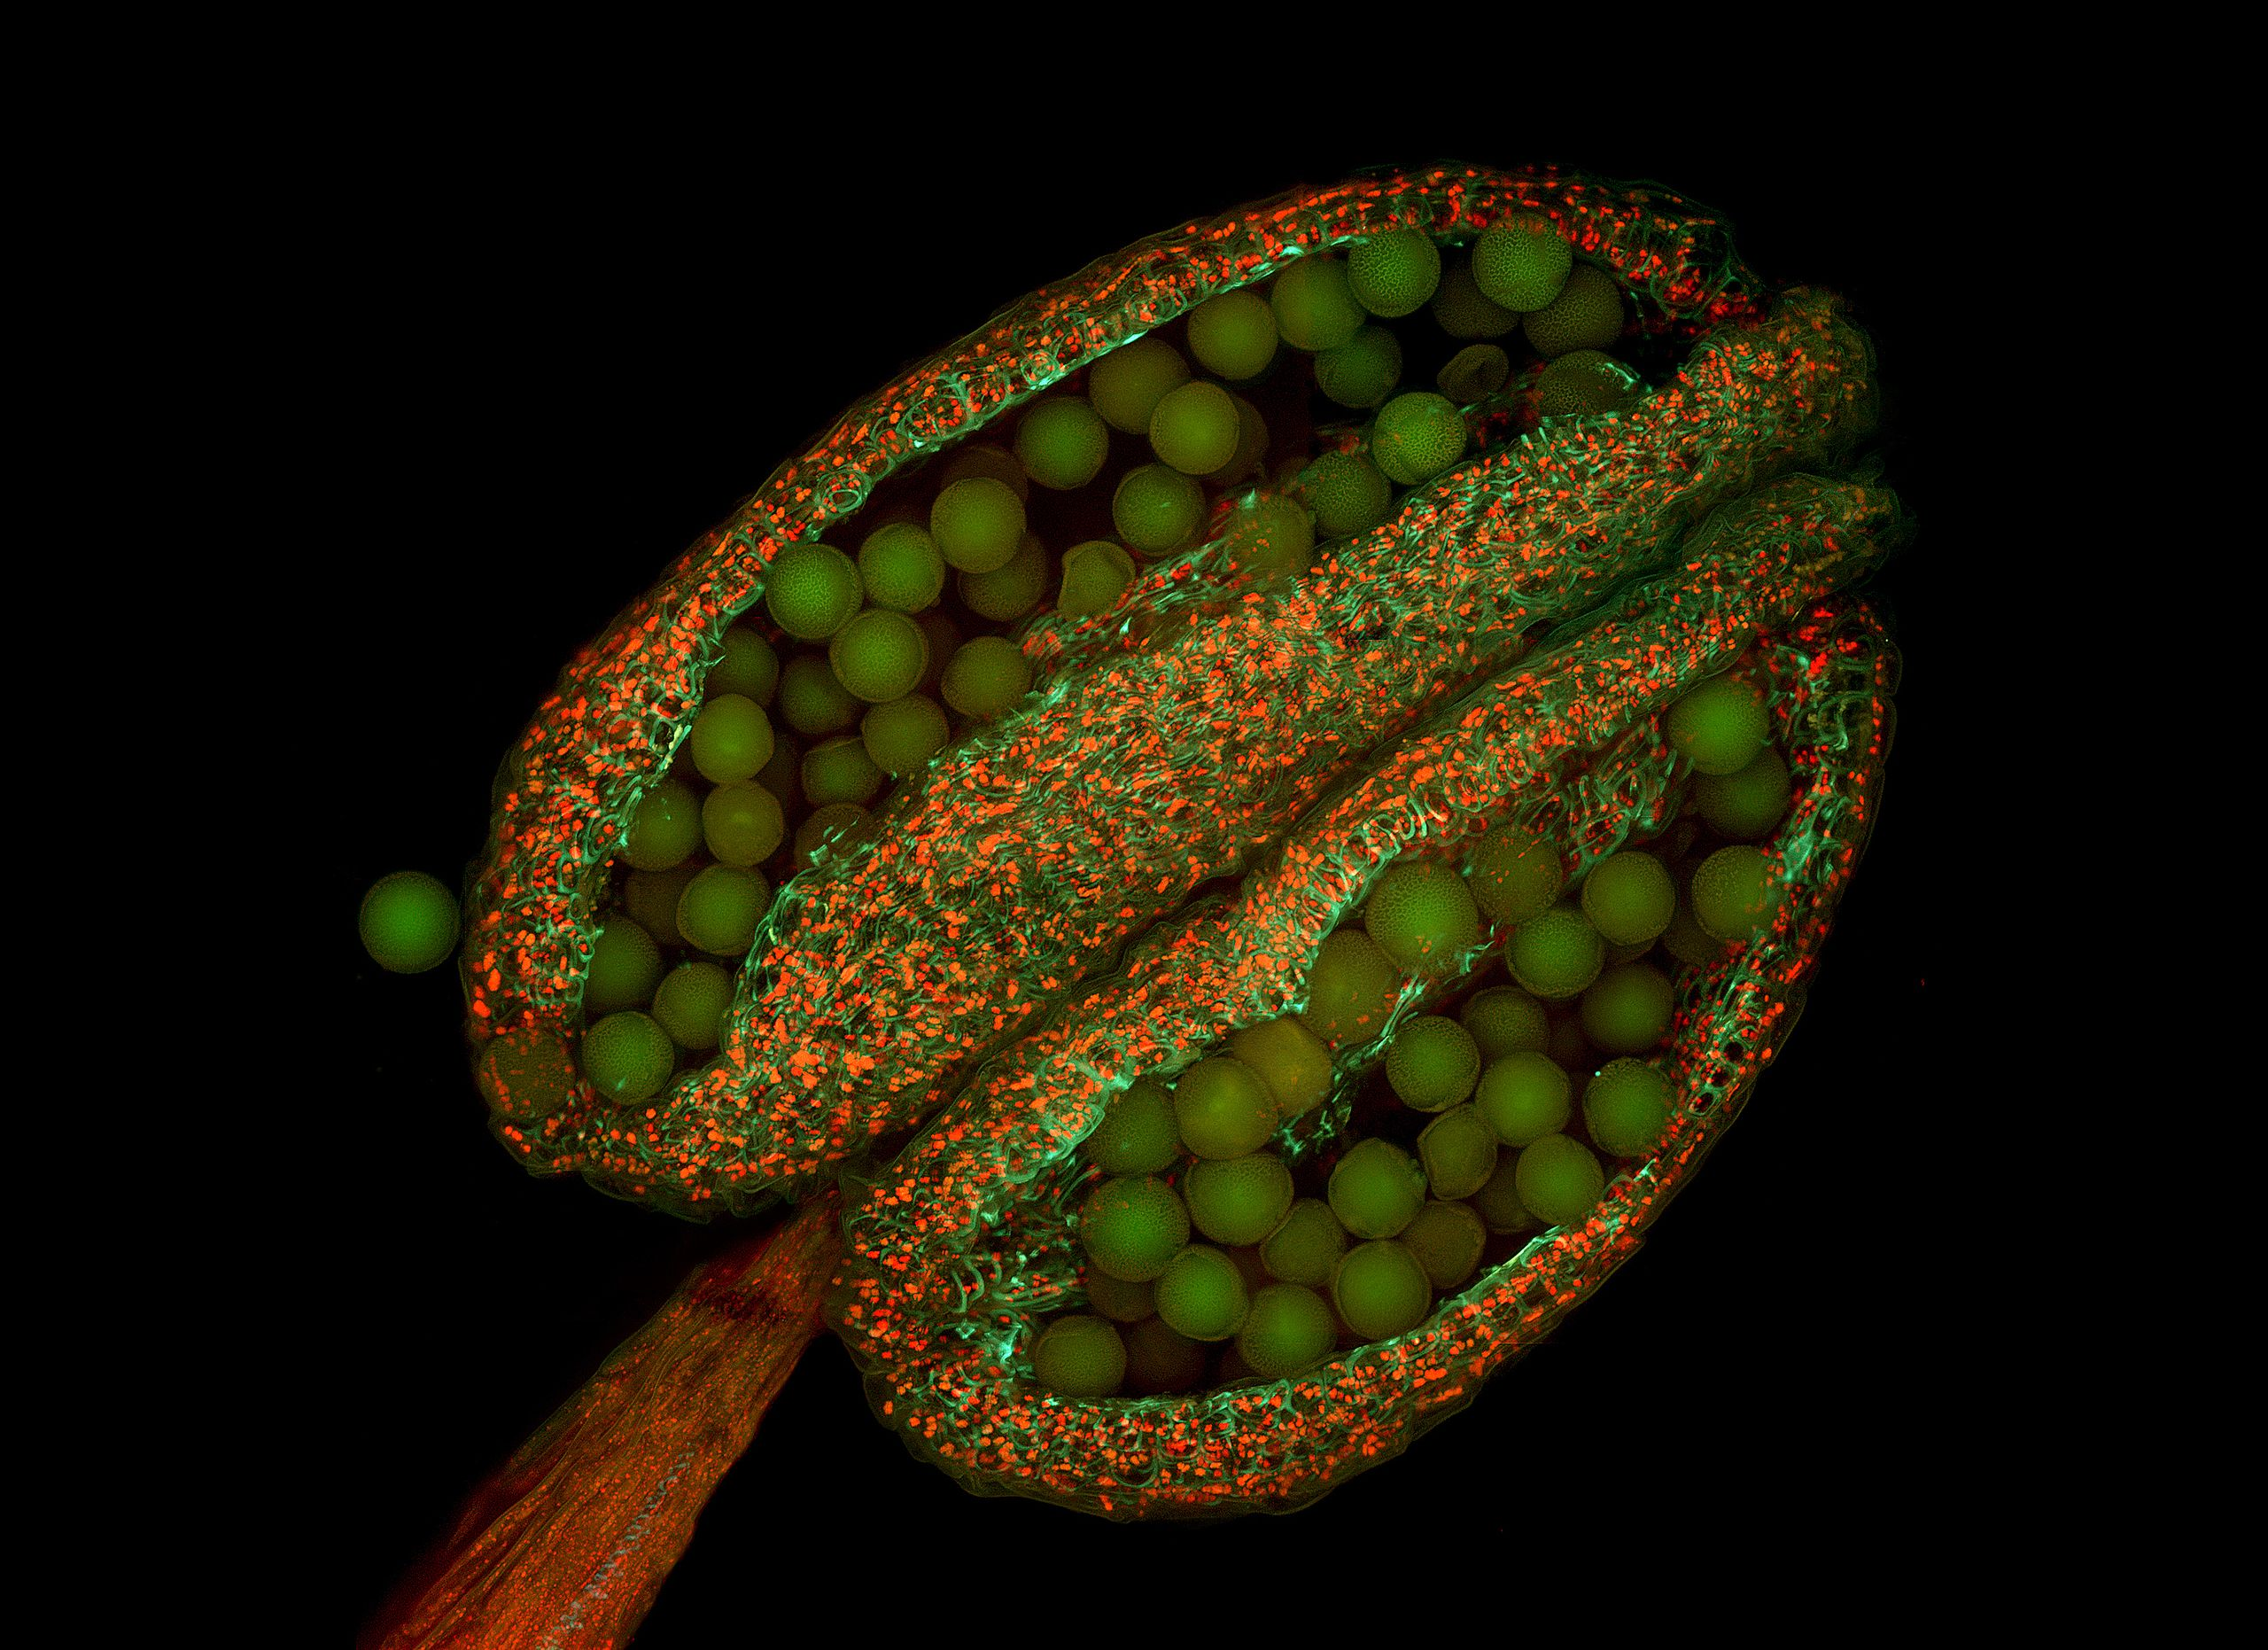
\includegraphics[width=\linewidth]{Tolmukapea.jpg}
% 	\caption{Anther of thale cress (Arabidopsis thaliana), fluorescence micrograph. Source: Heiti Paves, \href{https://commons.wikimedia.org/wiki/File:Tolmukapea.jpg}{https://commons.wiki-\\media.org/wiki/File:Tolmukapea.jpg}.}
% 	\label{fig:tcanther}
% \end{figure}

% Referencing a figure using its label: Figure \ref{fig:tcanther}.

% Aenean porttitor eros non pharetra congue. Proin in odio in dolor luctus auctor ac et mi. Etiam euismod mi sed lectus fringilla pretium. Phasellus tristique maximus lectus et sodales. Mauris feugiat ligula quis semper luctus. Nam sit amet felis sed leo fermentum aliquet. Mauris arcu dui, posuere id sem eget, cursus pulvinar mi. Donec nec lacus non lectus fermentum scelerisque et at nibh. Sed tristique, metus ac vestibulum porta, tortor lectus placerat lorem, et convallis tellus dolor eget ante. Pellentesque dui ligula, hendrerit a purus et, volutpat tempor lectus. Mauris nec purus nec mauris rhoncus pellentesque. Quisque quis diam sed est lacinia congue. Donec magna est, hendrerit sed metus vel, accumsan rutrum nibh.

% \begin{figure*} % Two column figure (notice the starred environment)
% 	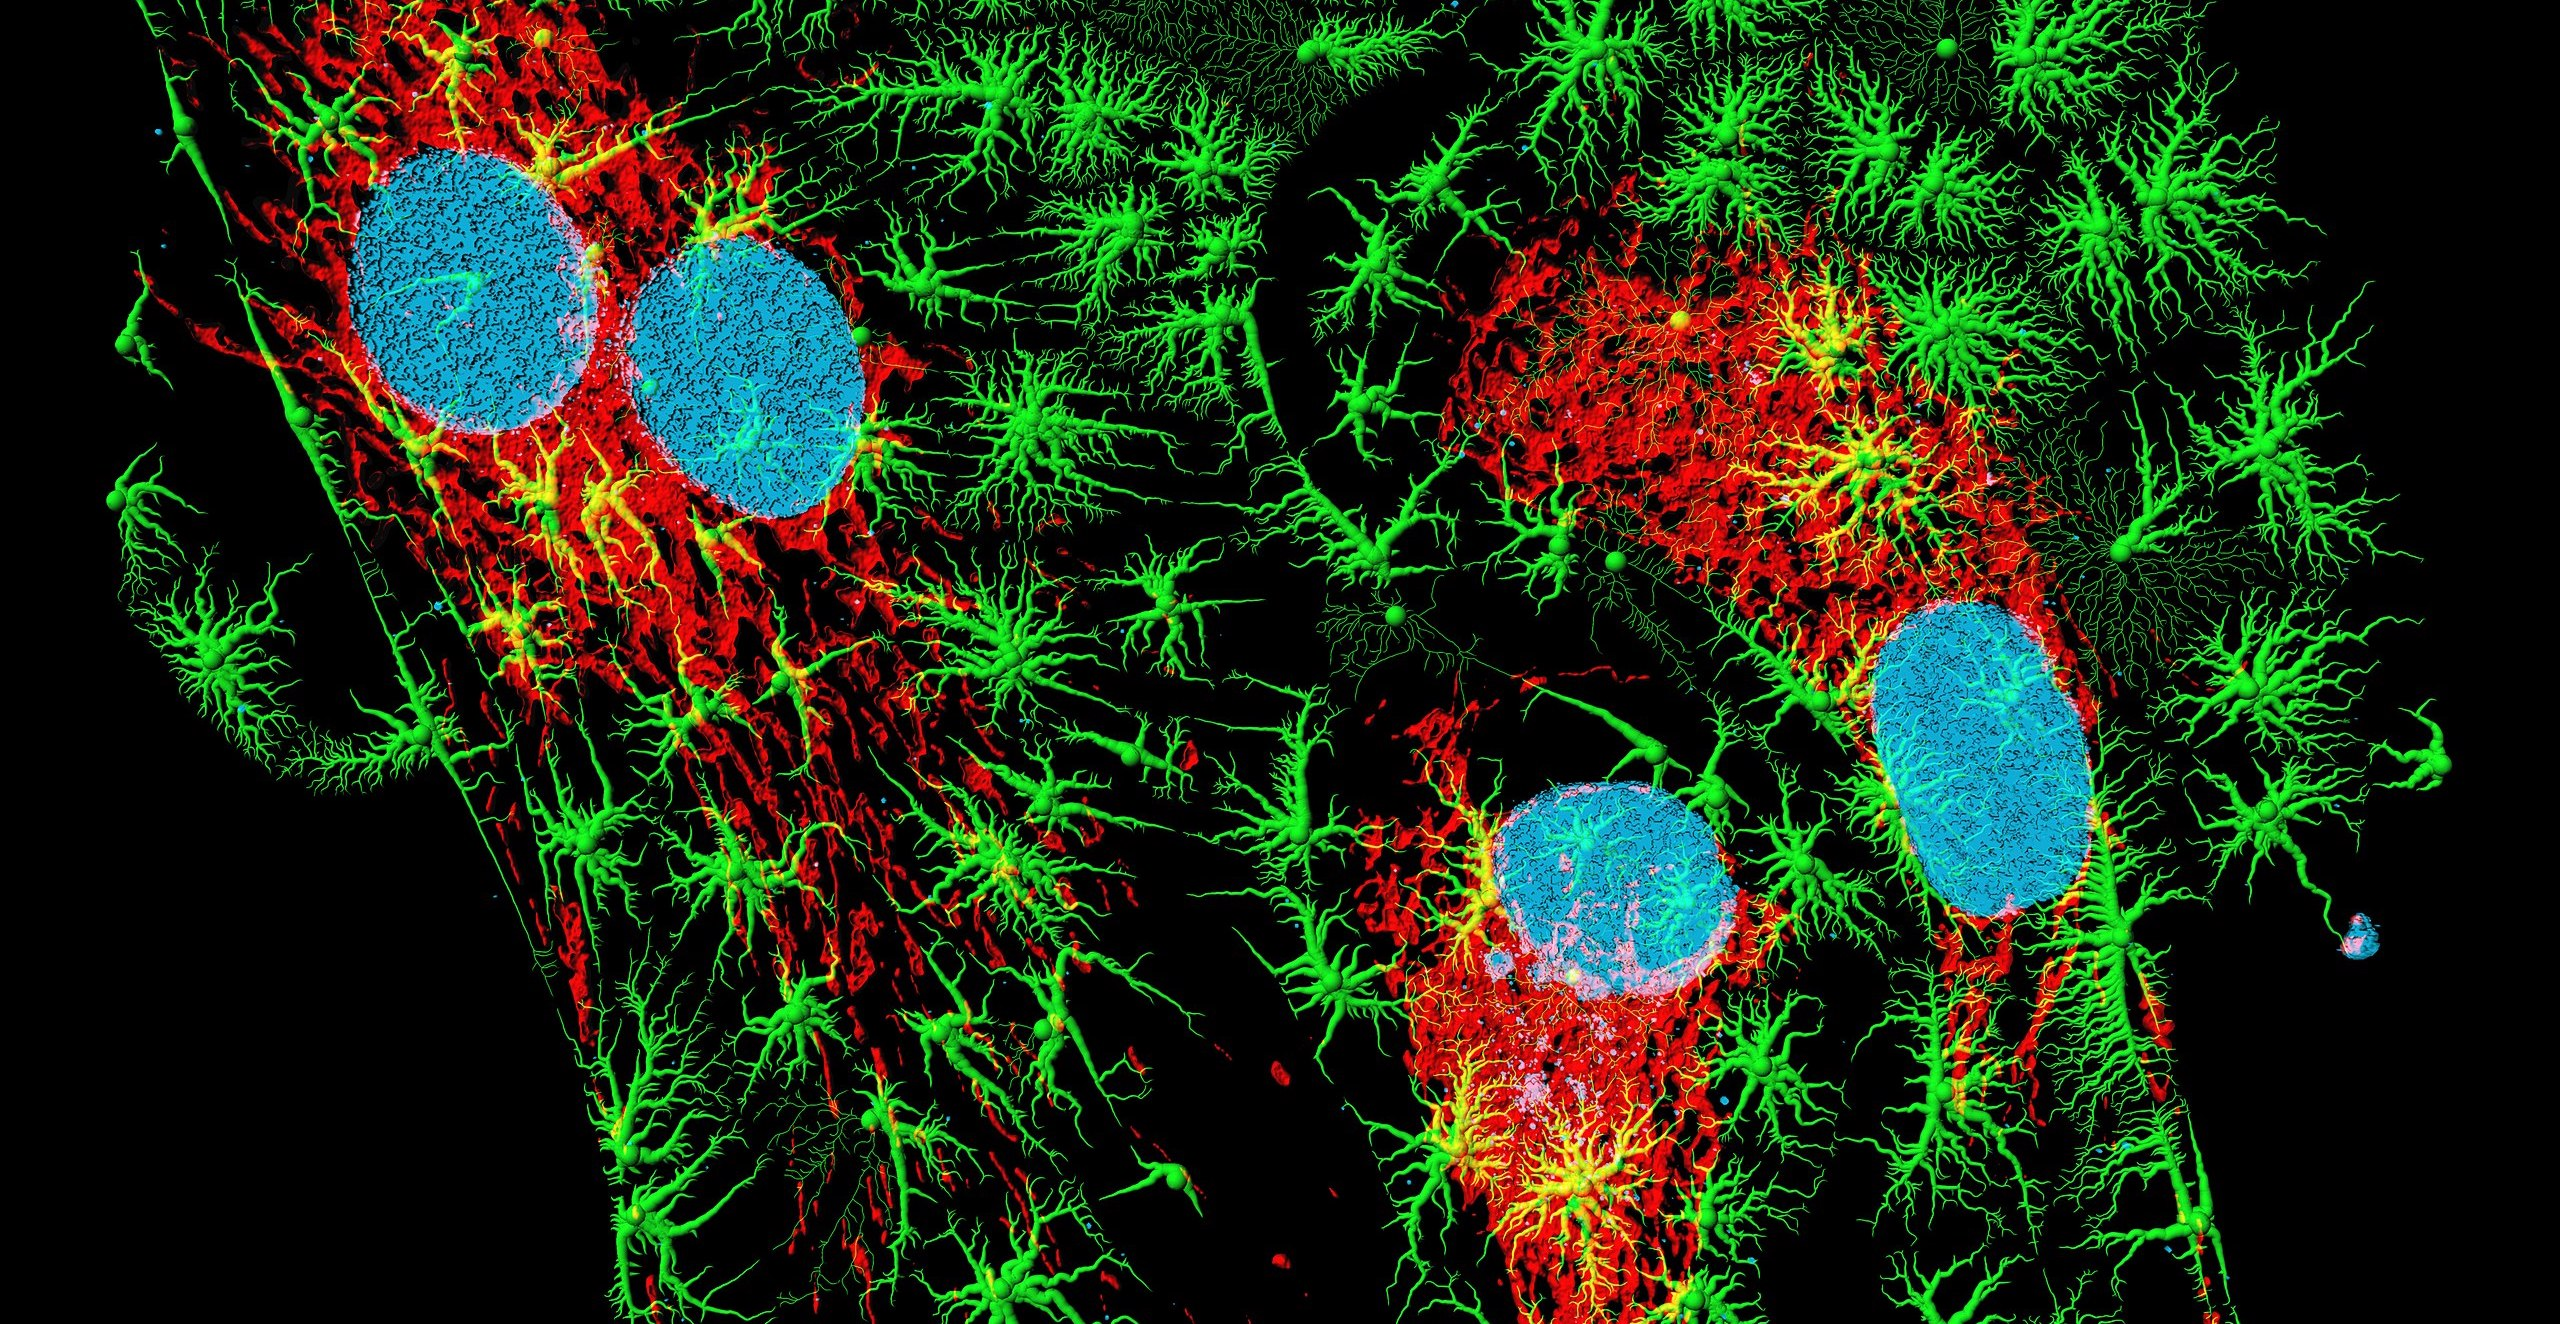
\includegraphics[width=\linewidth]{Fibroblastid.jpg}
% 	\caption{Bovine pulmonary artery endothelial cells in culture. Blue: nuclei; red: mitochondria; green: microfilaments. Computer generated image from a 3D model based on a confocal laser scanning microscopy using fluorescent marker dyes. Source: Heiti Paves, \href{https://commons.wikimedia.org/wiki/File:Fibroblastid.jpg}{https://commons.wikimedia.org/wiki/File:Fibroblastid.jpg}.}
% 	\label{fig:bpartery}
% \end{figure*}

% Orci varius natoque penatibus et magnis dis parturient montes, nascetur ridiculus mus. Etiam cursus lectus purus, tempus iaculis quam dictum tristique. Nam interdum sapien nec tempor mattis. Quisque id sapien nisi. Mauris vehicula ornare eros vel efficitur. Nulla consectetur, turpis quis fringilla tincidunt, mi neque iaculis lectus, vel commodo elit odio non ex. Duis facilisis, purus ac viverra iaculis, turpis lectus ultrices ante, ac vestibulum ligula magna in libero. Etiam tristique maximus lacinia. Vestibulum hendrerit, lacus malesuada laoreet blandit, sapien velit sollicitudin nunc, eu porttitor urna ligula at lorem. Aliquam faucibus eros in fermentum venenatis. Fusce consectetur congue pellentesque. Suspendisse at nisi sit amet est porttitor cursus. Cras placerat faucibus nunc, a laoreet justo dignissim sit amet.

% \subsection{International Support}

% \noindent àáâäãåèéêëìíîïòóôöõøùúûüÿýñçčšž

% \noindent ÀÁÂÄÃÅÈÉÊËÌÍÎÏÒÓÔÖÕØÙÚÛÜŸÝÑ

% \noindent ßÇŒÆČŠŽ

% \subsection{Links}

% This is a clickable URL link: \href{https://www.latextemplates.com}{LaTeX Templates}. This is a clickable email link: \href{mailto:vel@latextemplates.com}{vel@latextemplates.com}. This is a clickable monospaced URL link: \url{https://www.LaTeXTemplates.com}.

% %------------------------------------------------

\section{Measures of Success}
To evaluate the effecvtiveness of our film emulation we will emply qualitative and quantitative assessments. 

\subsection{Qualitative Evaluation}
% TODO: Adding film image properties
We will perform visual comparisons between our processed images and reference images to assess the effectiveness of our film emulation approach. These comparisons will focus on certain analog imaging properties such as $\textbf{[insert some film image properties]}$. By examining these specific attributes, we can evaluate how successful our algorithm reproduced the distinctive aesthetic properties of film. Finally, a successful film emulation implementation would not have any unintended artifacts such as ghosting from the registration process or unusual transitions between light and dark.

This statement requires citation \autocite{Smith:2023qr}. This statement requires multiple citations \autocite{Smith:2023qr, Smith:2024jd}. This statement contains an in-text citation, for directly referring to a citation like so: \textcite{Smith:2024jd}.

\subsection{Quantitative Evaluation}

Using OpenCV and NumPy, we will calculate the dynamic range of our processed images to measure how well the HDR functionality has been implemented. 
In addition to calculating the dynamic range we will create difference maps comparing our normalized HDR images to the original input images. This will demonstrate our algorithm’s ability to preserve information while adding the film characteristics. Ideally, we should be able to compress our HDR image back to the original digital image exposure ranges.
 
An additional metric to evaluate our HDR composition process and image set will be to compare the image response curve generated by the Debevec algorithm to the known response curve of our chosen film stock and digital camera to ensure that our method is accurately compositing exposures.


\section{Goals}

The primary objective of our project is to develop algorithms that emulate the distinctive characteristics of photographic film and increase the dynamic range of digital images. Through this work, we aim to deepen our understanding of film response characteristics particularly how film cameras interpret light intensity in comparison to digital sensors. By implementing film processing techniques we will create algorithms which address the limitations of digital image capturing using modern photographic technology and create visually appealing images. 

\section{Potential Challenges}

First, working with RAW image data presents significant complexity since OpenCV does not directly support RAW images. We will need to implement preprocessing techniques so that the image is in a format compatible with OpenCV while ensuring the full dynamic range from the digital sensor is preserved. Another challenge we foresee is accurately reproducing film response characteristics. Film has a non-linear response light which is complex to accurately mathematically model. Finally, sensors in digital cameras vary and different camera sensors will result in different response curves. This may require device-specific algorithms so that our film emulation remains accurate. 

%----------------------------------------------------------------------------------------
%	 REFERENCES
%----------------------------------------------------------------------------------------

\printbibliography % Output the bibliography

%----------------------------------------------------------------------------------------

\end{document}
